\documentclass[12pt,a4paper]{article}
\usepackage[margin=2cm]{geometry}
\usepackage[spanish]{babel}
\usepackage{graphicx, multicol, latexsym, amsmath, amssymb}
\usepackage{array}
\usepackage{tabularx}
\usepackage{setspace}
\usepackage{titlesec}
\usepackage{subcaption}
\usepackage{float}
\usepackage{url}
\usepackage{hyperref}

% Ajuste de espacio entre secciones
\titlespacing*{\section}{0pt}{0.5em}{0.5em}

\renewcommand{\arraystretch}{1.3}

\begin{document}

% ---------------------------
% Encabezado con datos
% ---------------------------
\noindent
\begin{tabularx}{\textwidth}{|X|X|}
\hline
\textbf{Carné:} 2020045294 & \textbf{Nombre:} Justin Jaffeth Corea Masís \\
\hline
\textbf{Correo:} coreajustin288@estudiantec.cr & \textbf{Semana:} 2 del 20/08/2025 al 27/08/2025 \\
\hline
\end{tabularx}

\vspace{0.5cm}

% ---------------------------
% Tabla de actividades
% ---------------------------
\section*{Actividades realizadas}

% \begin{tabularx}{\textwidth}{|>{\raggedright\arraybackslash}p{8cm}|c|c|}
\begin{tabularx}{\textwidth}{|>{\raggedright\arraybackslash}p{12cm}|c|c|}
\hline
\textbf{Actividad} & \textbf{Fecha} & \textbf{Horas} \\
\hline
Realicé la conexión al clúster Kabré, instalé los paquetes necesarios e inicié prueba para YOLO & 21/08/2025 & 8 \\
\hline
Continué la redacción del capítulo 1 de la tesis & 22/08/2025 & 6 \\
\hline
Investigué cuál será el código a usar para entrenar reconocimiento de placas & 23/08/2025 & 4 \\
\hline
Corrección de imágenes y definición de casos extra de imágenes sintéticas & 23/08/2025 & 2 \\
\hline
Ejecución de pruebas con otras versiones de YOLO y corregí algunos problemas con el clúster & 24/08/2025 & 4 \\
\hline
Pruebas para preparando código para reconocimiento de placas & 25/08/2025 & 8 \\
\hline
Redefinir estrategia a usar para reconocimiento de placas & 26/08/2025 & 10 \\
\hline
\end{tabularx}

\vspace{1cm}

% ---------------------------
% Firma
% ---------------------------
\noindent
\textbf{Firma del Profesor Asesor:}

\vspace{2cm}

\noindent\rule{8cm}{0.4pt}  
Nombre y firma

\newpage

\section{Detección de placas}

\subsection{Matrices de confusión}

\begin{figure}[H]
	\centering
	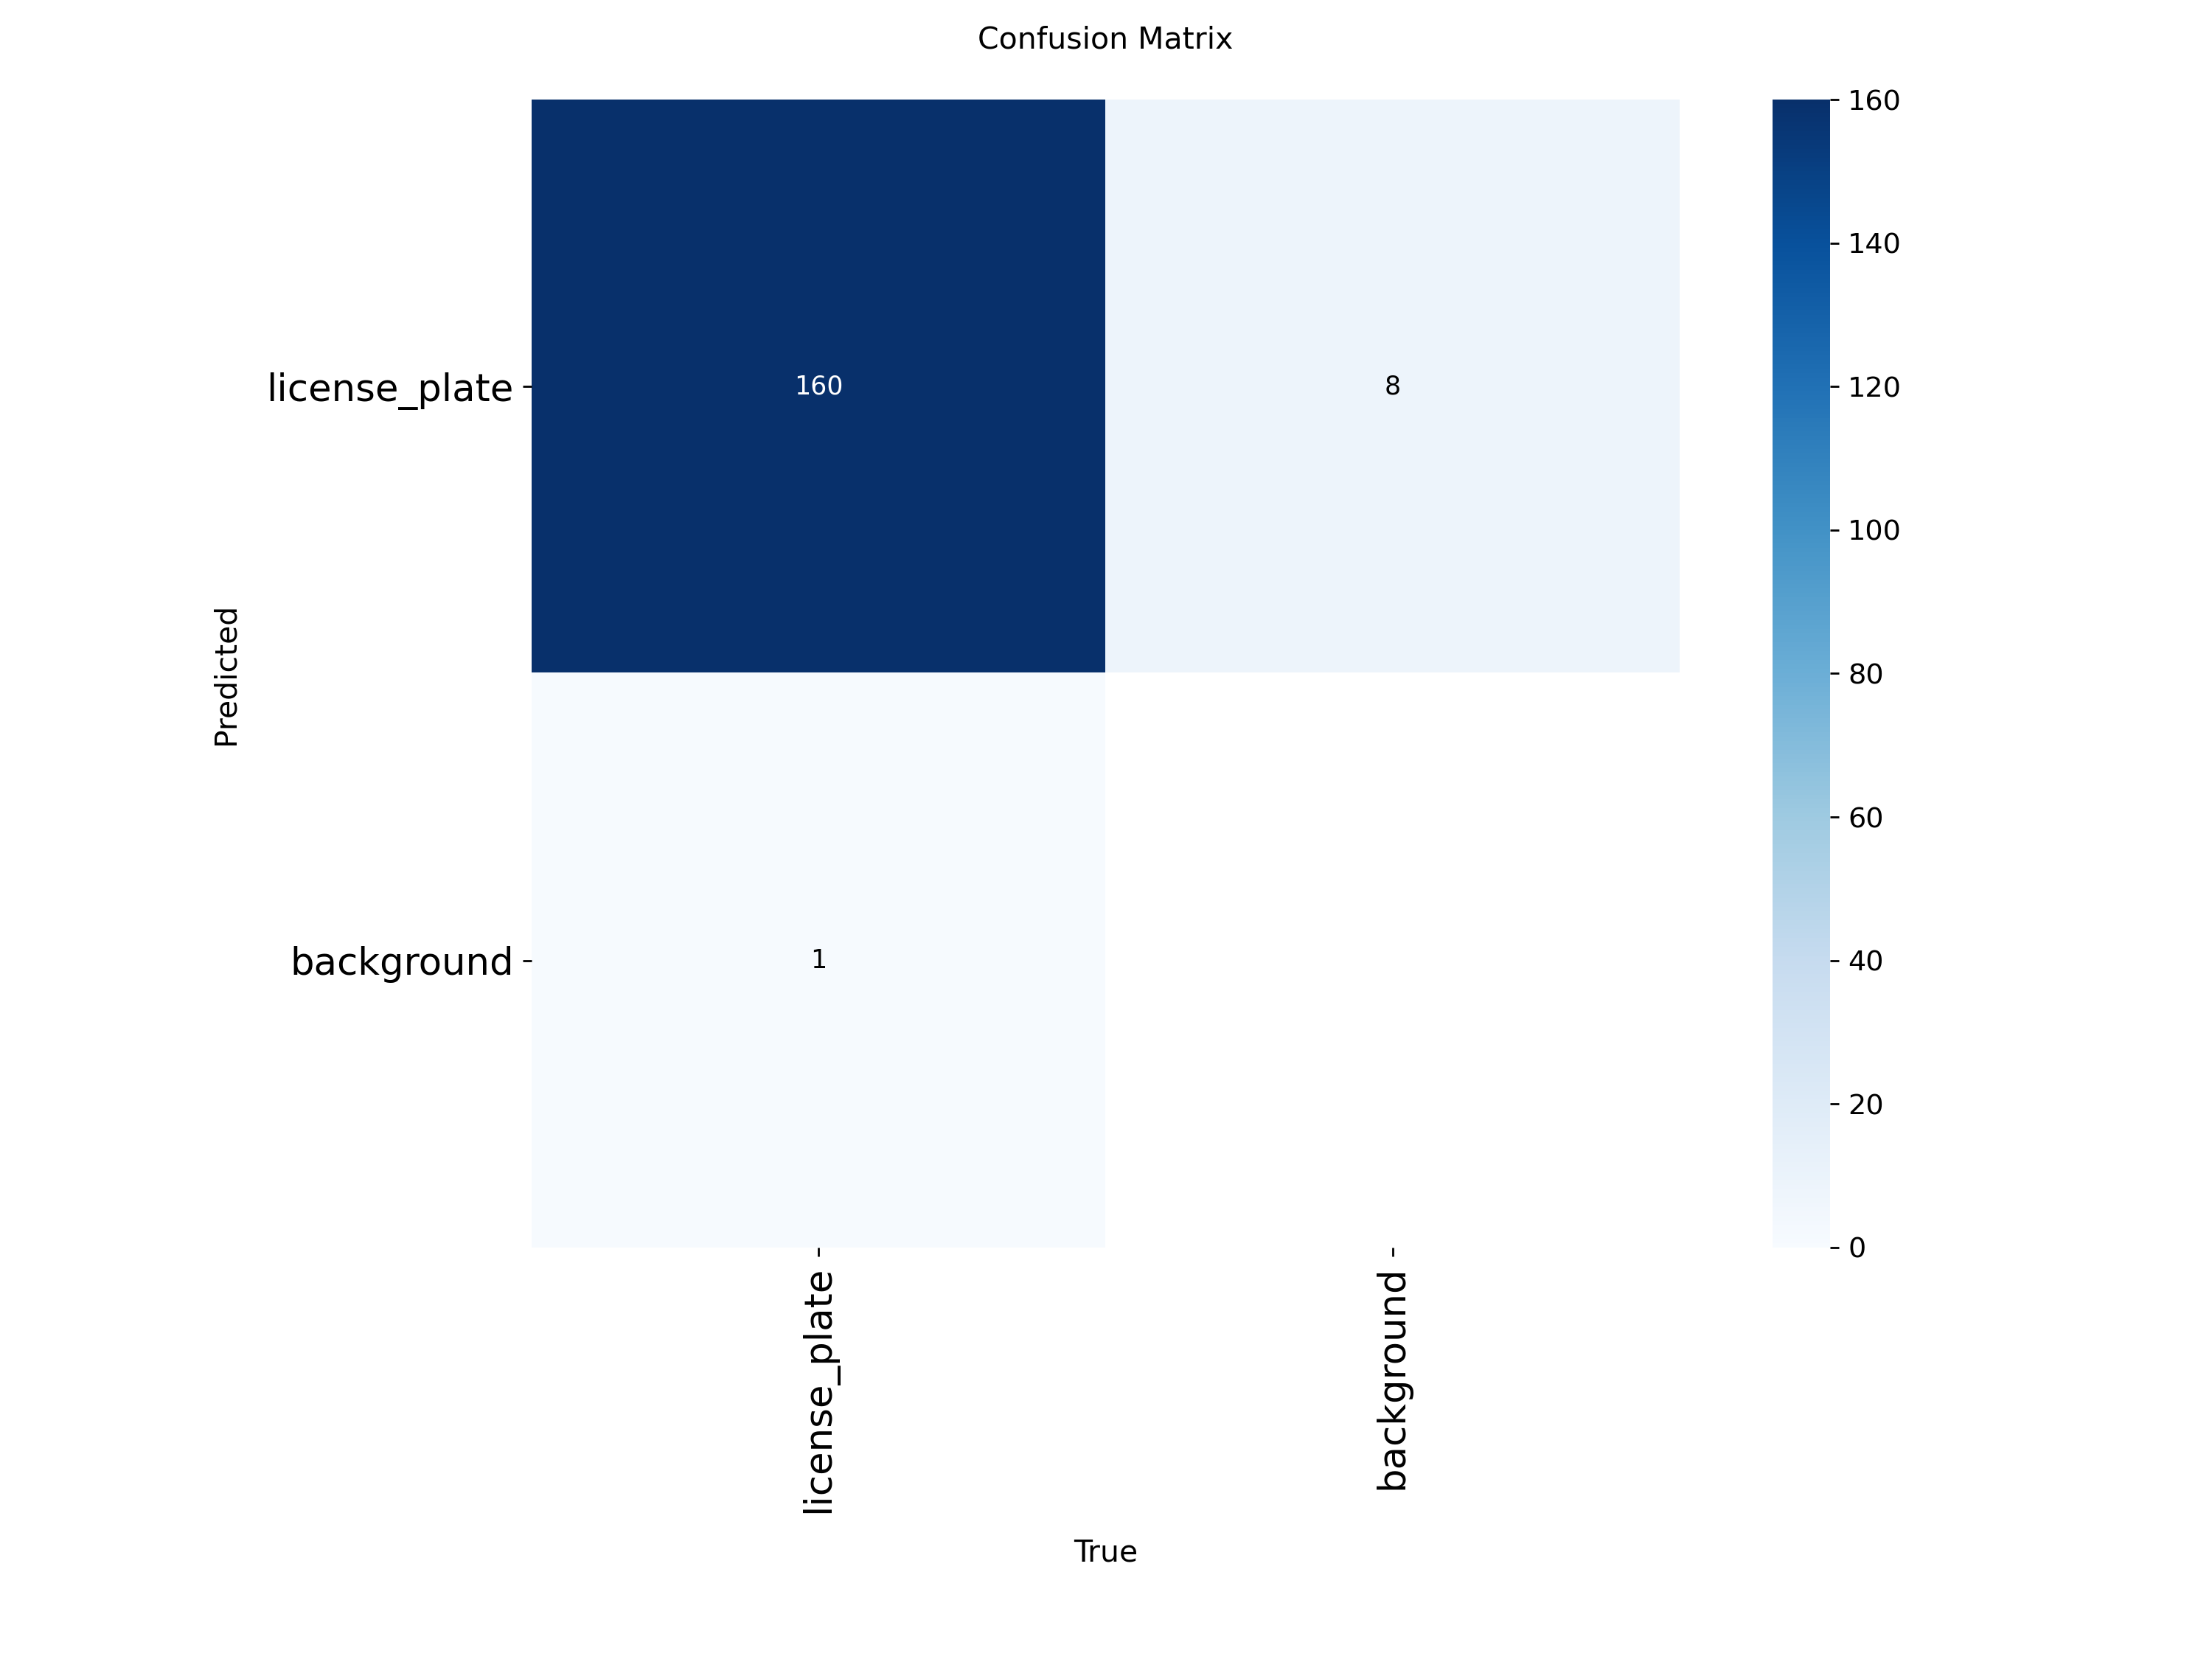
\includegraphics[width=0.8\textwidth]{../cap1/fig/proy/confusion_matrix-new-model.png}
	\caption{Mejor modelo con YOLOv11}
\end{figure}

\begin{figure}[H]
	\centering
	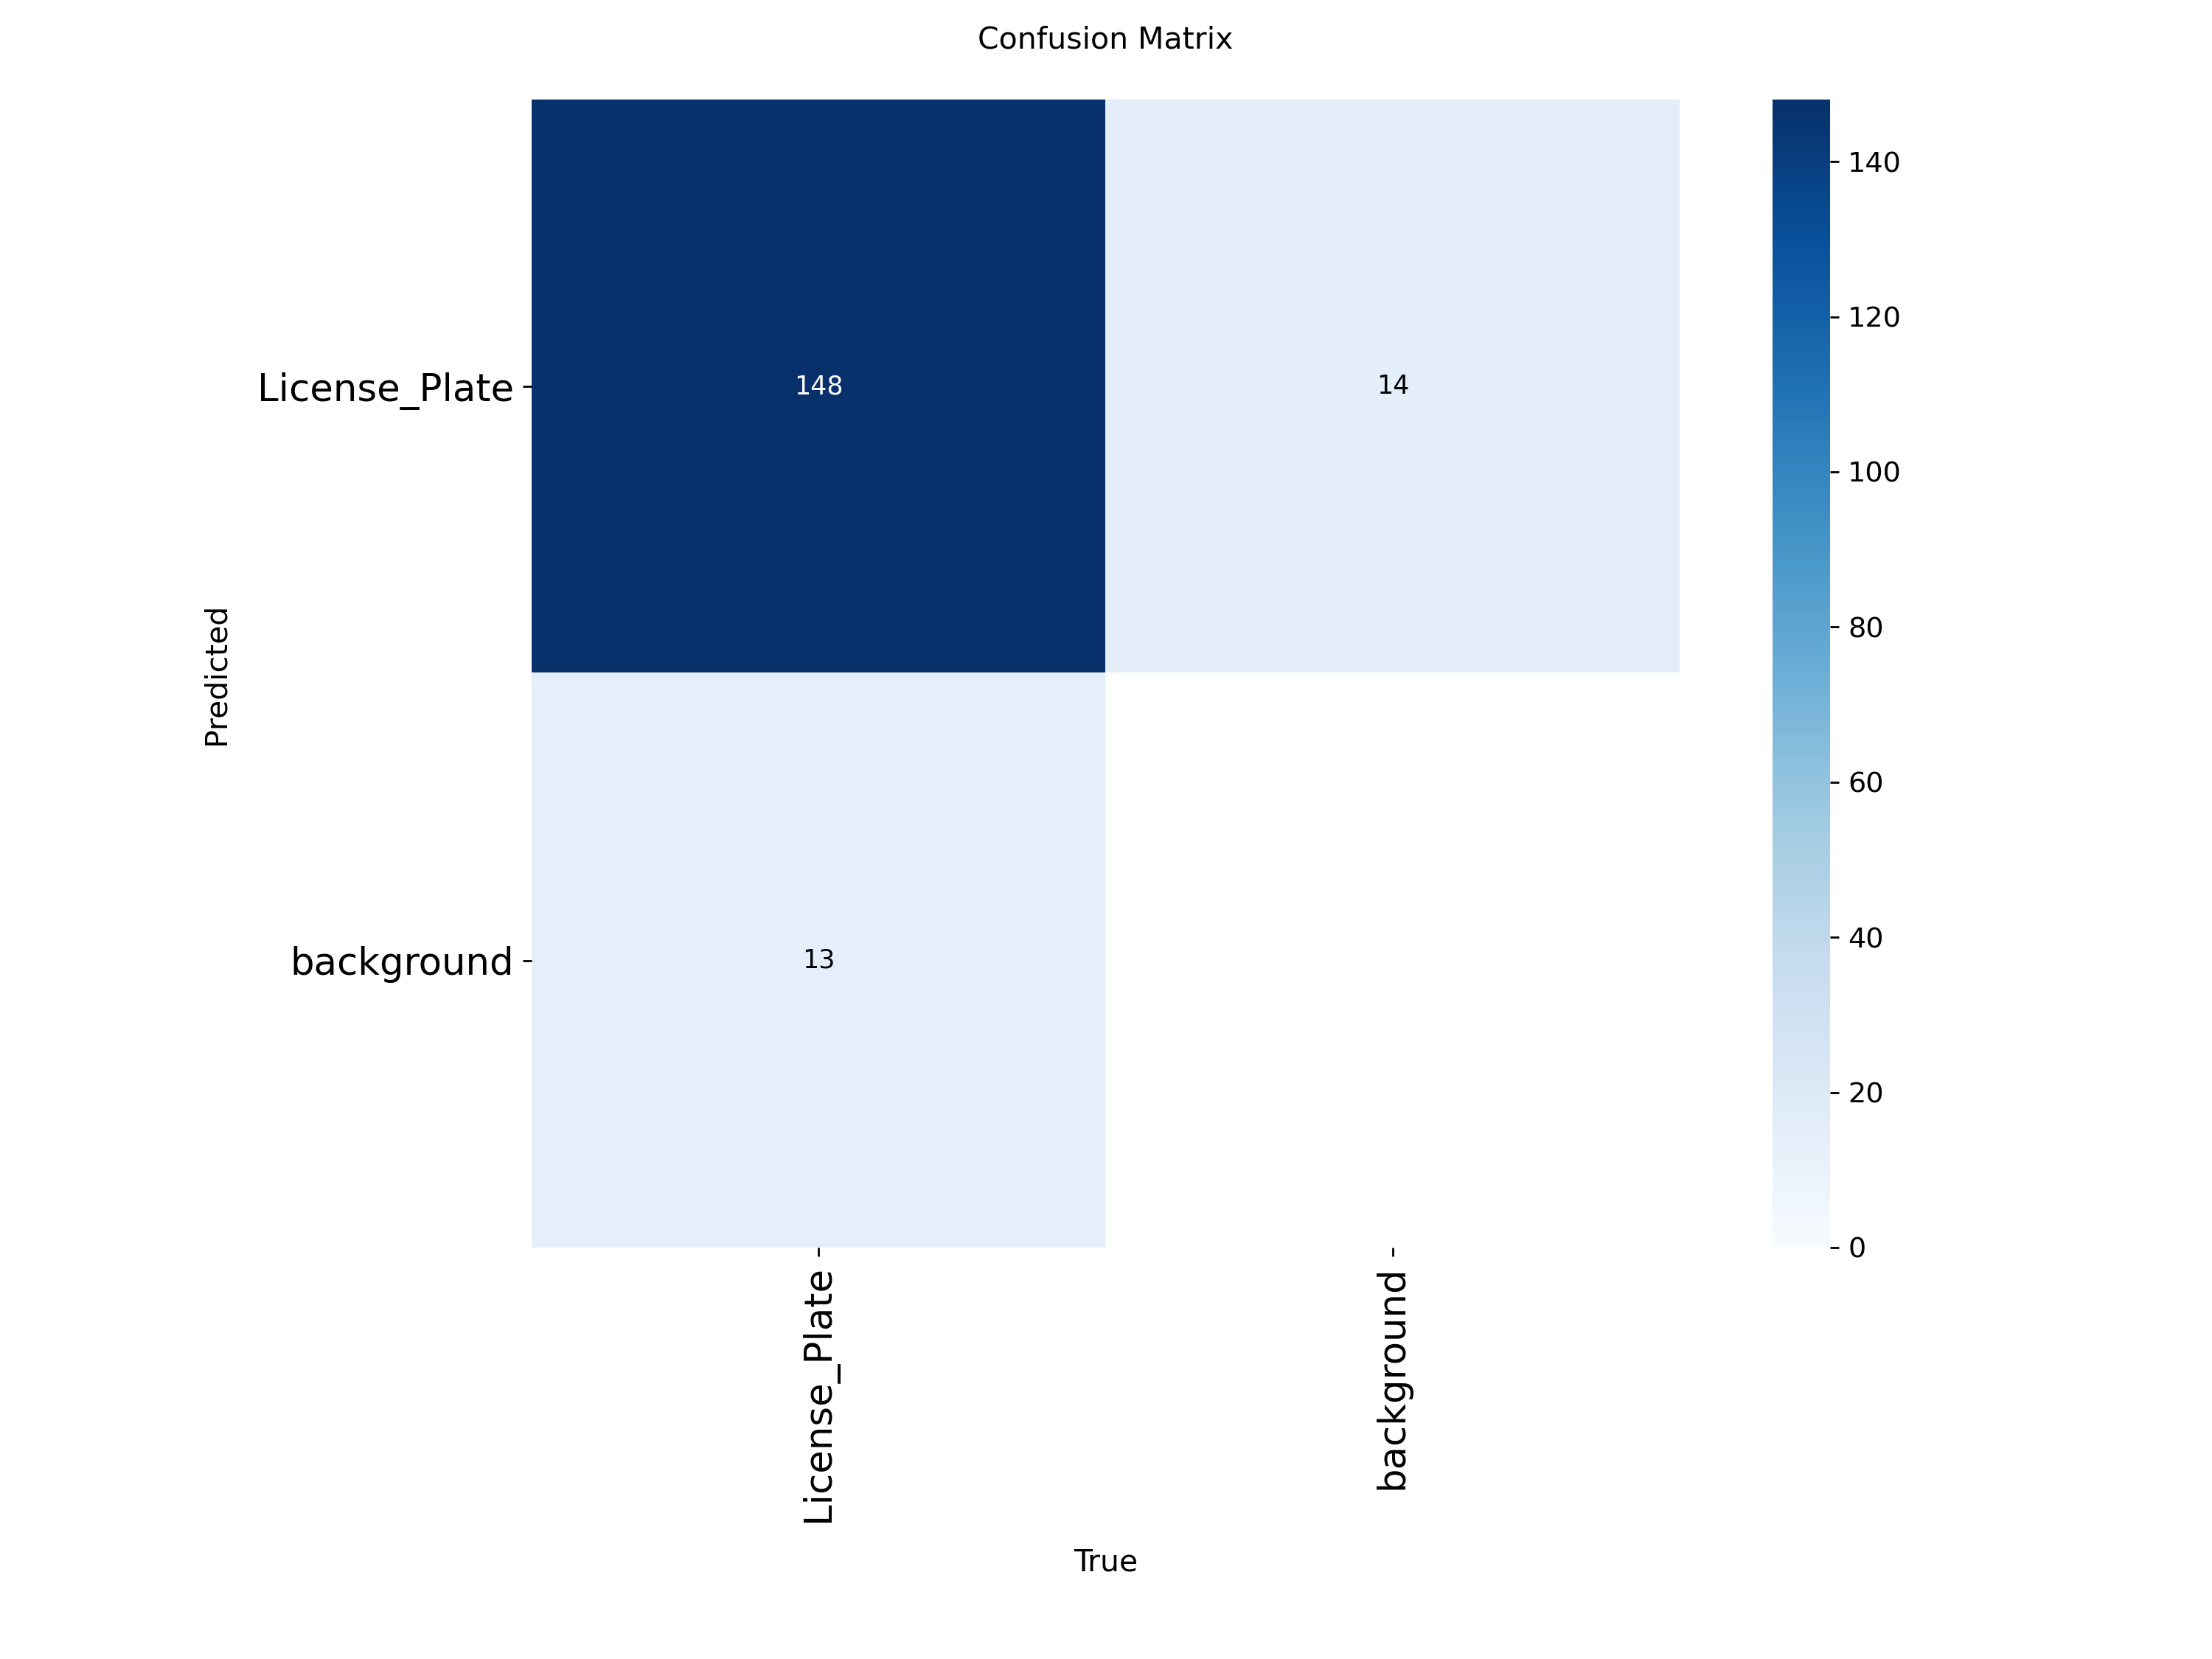
\includegraphics[width=0.8\textwidth]{../cap1/fig/proy/confusion_matrix-old-model.png}
	\caption{Modelo antiguo}
\end{figure}

\begin{figure}[H]
	\centering
	\includegraphics[width=0.8\textwidth]{../../src/runs/eval/pretrained/confusion_matrix.png}
	\caption{Modelo base sin ajuste}
\end{figure}

\subsection{Evaluación en batch}

\begin{figure}[H]
	\centering
	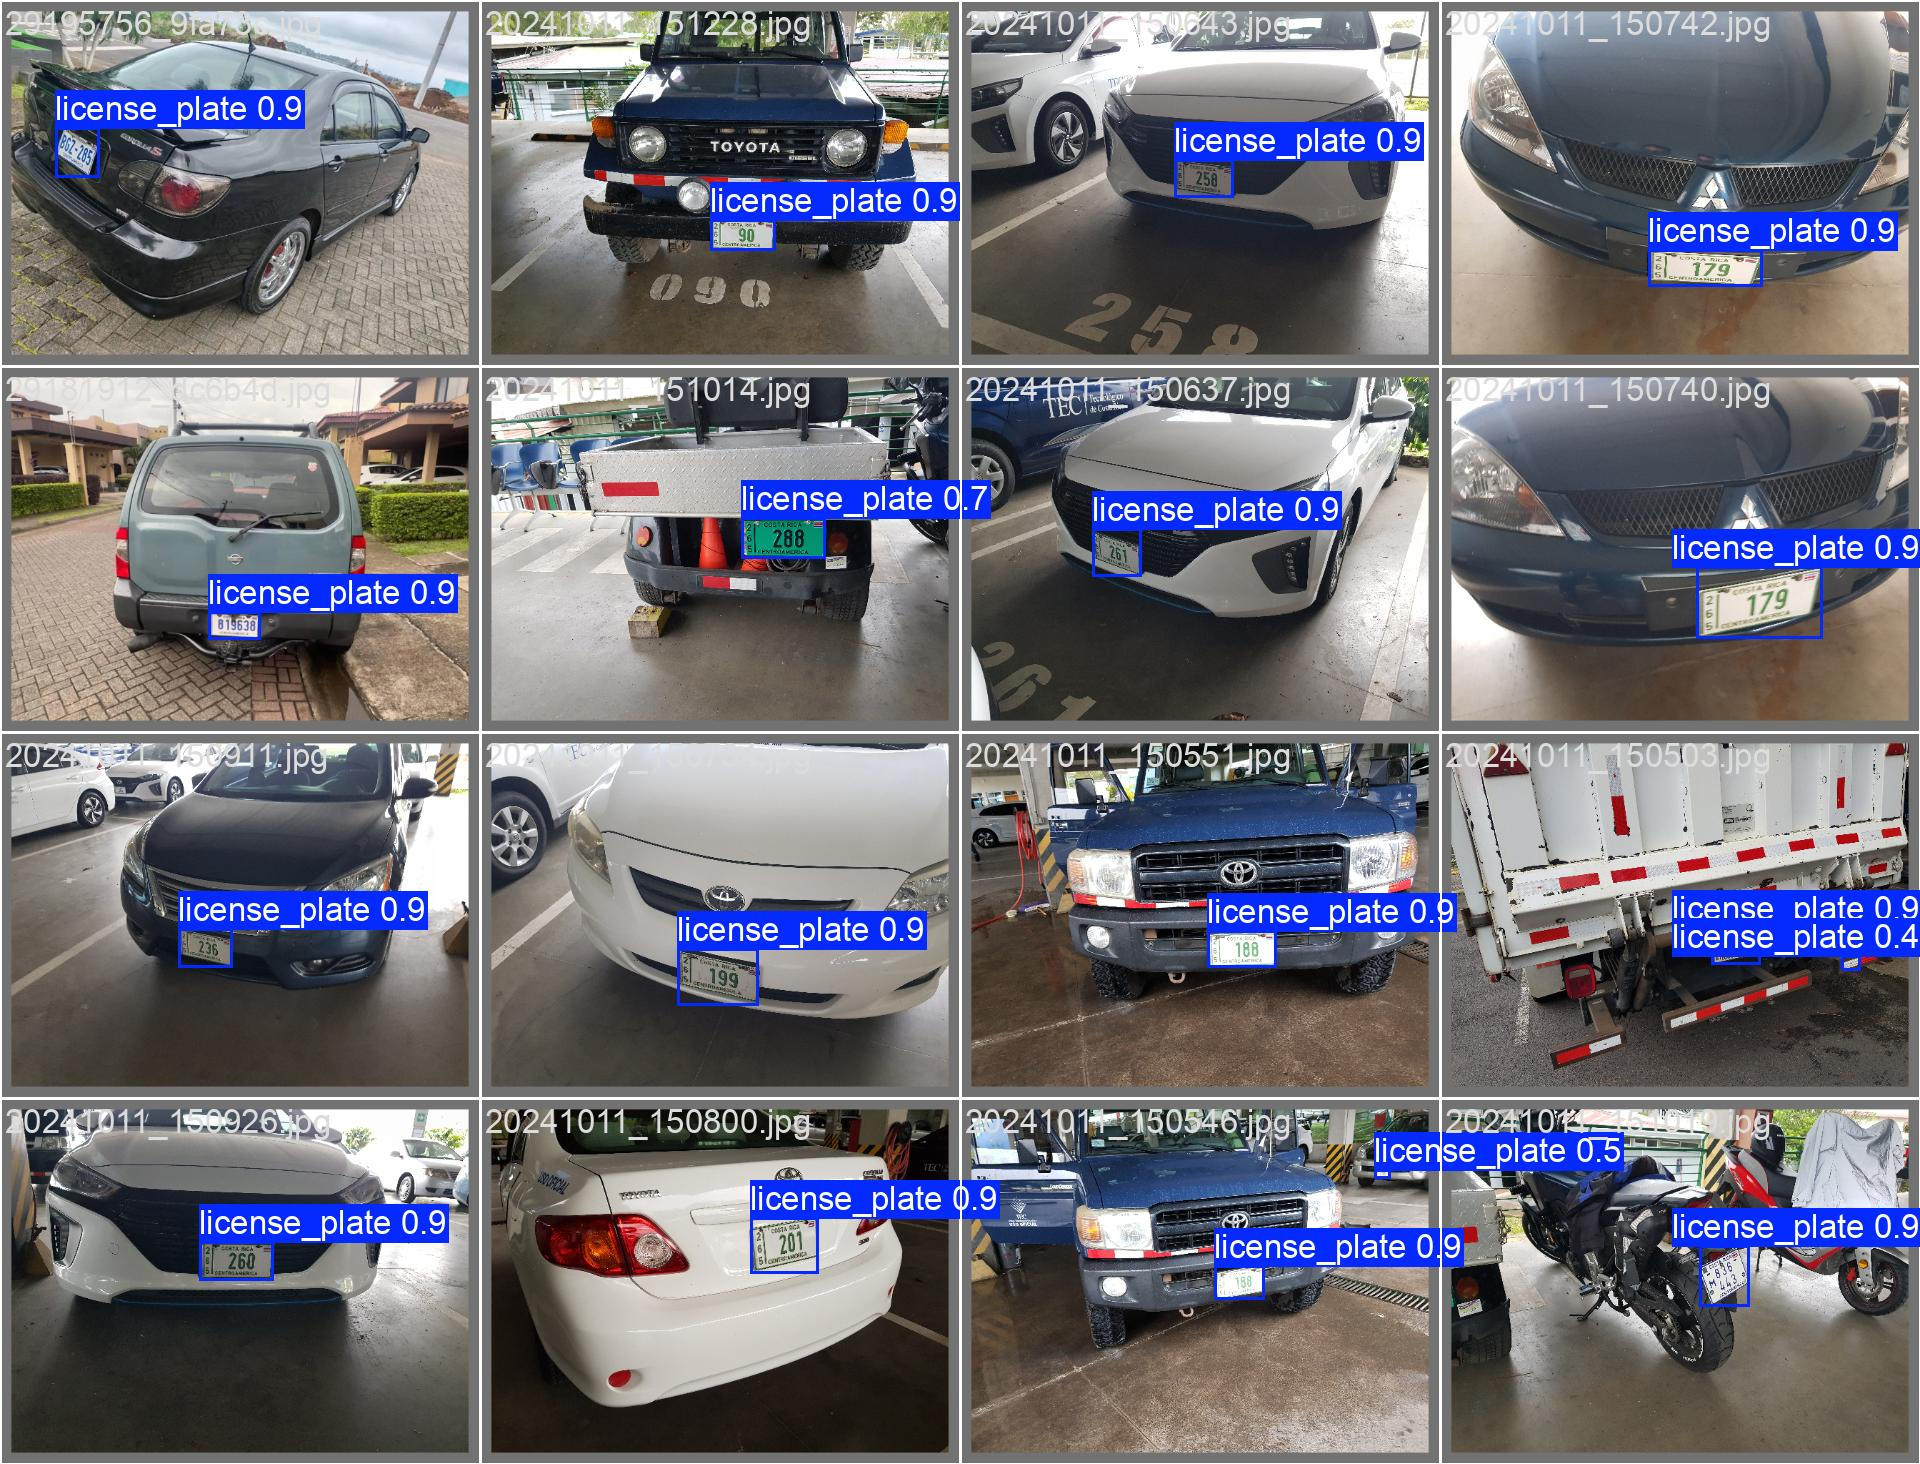
\includegraphics[width=0.8\textwidth]{../cap1/fig/proy/ejemplo-deteccion-placas.jpg}
	\caption{Mejor modelo con YOLOv11}
\end{figure}

\begin{figure}[H]
	\centering
	\includegraphics[width=0.8\textwidth]{../../src/runs/eval/old_model/val_batch0_pred.jpg}
	\caption{Modelo antiguo}
\end{figure}

\begin{figure}[H]
	\centering
	\includegraphics[width=0.8\textwidth]{../../src/runs/eval/pretrained/val_batch0_pred.jpg}
	\caption{Modelo base sin ajuste}
\end{figure}

El modelo base de YOLO no tiene clase placas, por eso no reconoce nada.
El modelo nuevo es más preciso, que el anterior.

\section{Reconocimiento de placas}
Para esto escogí tres opciones, pero no logré hacer funcionar ninguno de momento:

\begin{itemize}
	\item \textbf{\href{https://github.com/mesakarghm/LPRNET.git}{LPRNet}}: Pero ya está algo 
		viejo. Lo probé y hay que cambiar bastante código, y cambiar formato de etiquetas.

	\item \textbf{\href{https://github.com/PaddlePaddle/PaddleOCR.git}{PaddleOCR}}.
		Otros proyecto de reconocimiento de placas lo usan y es mejor que EasyOCR, 
	pero tras muchas horas intentando no logré hacerlo funcionar en el clúster del CENAT. Da muchos errores
		de versiones de diferentes paquetes.

	\item \textbf{\href{https://github.com/wulb97/CLPRNet.git}{CLPRNet}}: Está bastante reciente.
		Pero hay que cambiar demasiadas cosas. Este parece muy bueno.
		Estoy intentando reescribir un poco el código para ajustarlo a mis necesidades.
\end{itemize}

\end{document}
